\fakesection{Function Estimation and Time Series Prediction}{\hfill\small\texttt{/src/session\_2/.m}}

\fakesubsection{Support vector machine for function estimation}{}

Two datasets are experimented with in figure \ref{functionestimation}. The first exists of 20 points lying on a slope. Therefore one can expect the linear kernel (which generates a linear model) to outperform the others. The second (non-linear) dataset is more challenging such that other kernels which enable the SVM to model the non-linearities have to be used instead. 

\par From the problem statement 
$$\min_{w,b,\xi,\xi^*}\frac{1}{2}w\cdot w^T+C\cdot\sum_{k=1}^N\xi+\xi^*$$
where $\xi,\xi^*$ are slack variables representing deviation from the so-called \textit{$\epsilon$-insensitive tube} it can be deduced that the $C$ (the \textit{bound}) plays the usual role of a regularisation parameter, prioritising either the smoothness of the model or how much it fits the data (i.e. minimising the slack variables). $C=0$ leads to simple horizontal lines for the linear kernel which express the view that the two input features $x_1$ and $x_2$ aren't related. The $\epsilon$ parameter controls the width of the tube in which the data points are made to lie. A larger value decreases the number of support vectors and makes the model less accurate.

\par The formulation resembles that of a least squares fit with Thikonov regularisation but the $\epsilon$-insensitive tube makes for a different loss function that encourages sparsity and since the problem is turned into a constraint optimisation problem a dual form can be expressed for which one can apply the kernel trick to be able to model any nonlinearities.

\begin{figure}[h]
\centering
\subfloat[Linear kernel.]{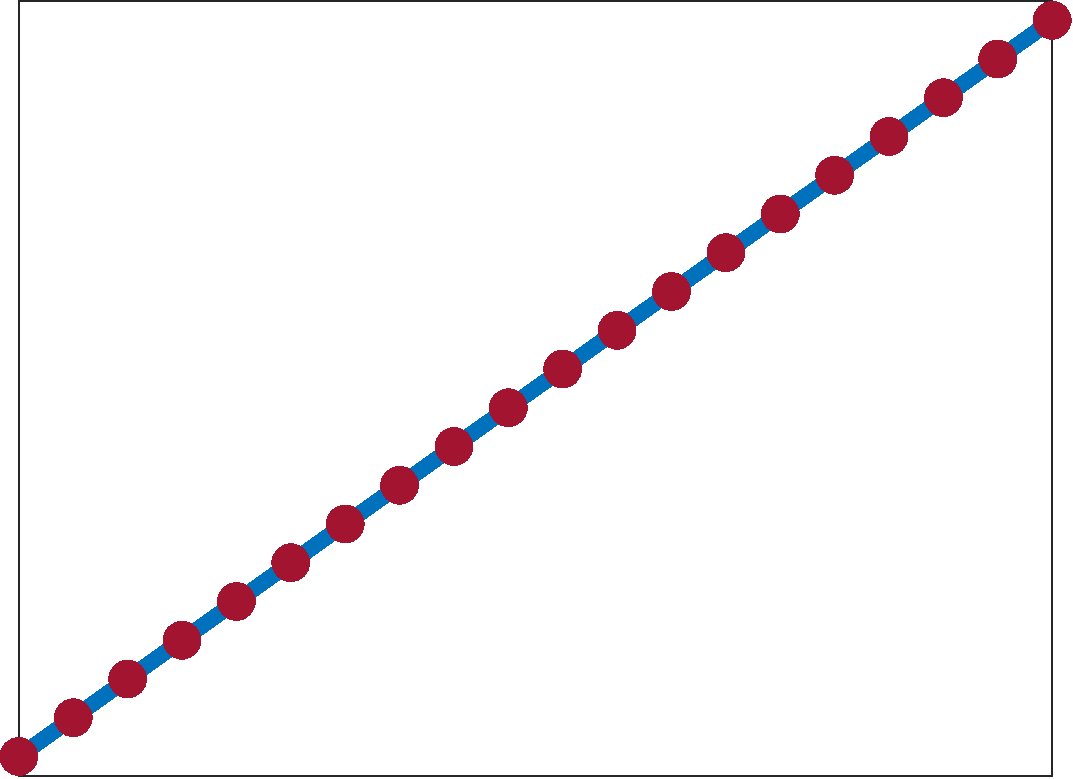
\includegraphics[width=0.16\textwidth]{../src/figures/estimation/gui_linear}}\qquad
\subfloat[Polynomial kernel, $\delta=3$.]{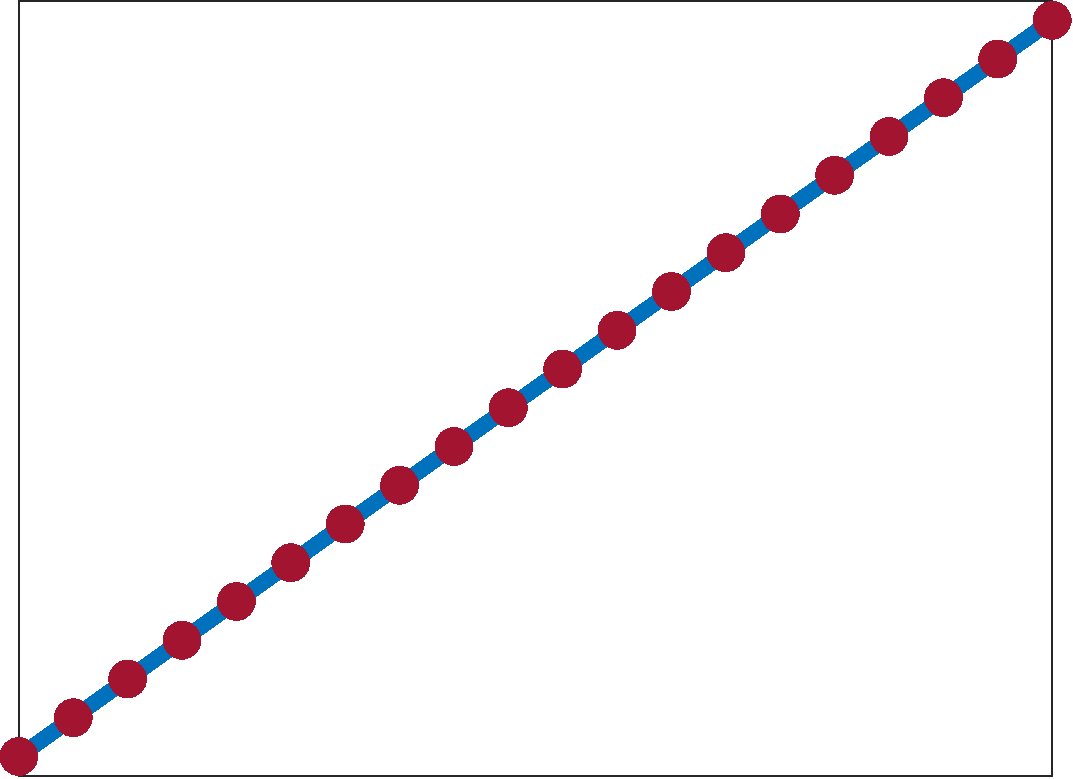
\includegraphics[width=0.16\textwidth]{../src/figures/estimation/gui_polynomial}}\qquad
\subfloat[RBF kernel, $\sigma^2=1$.]{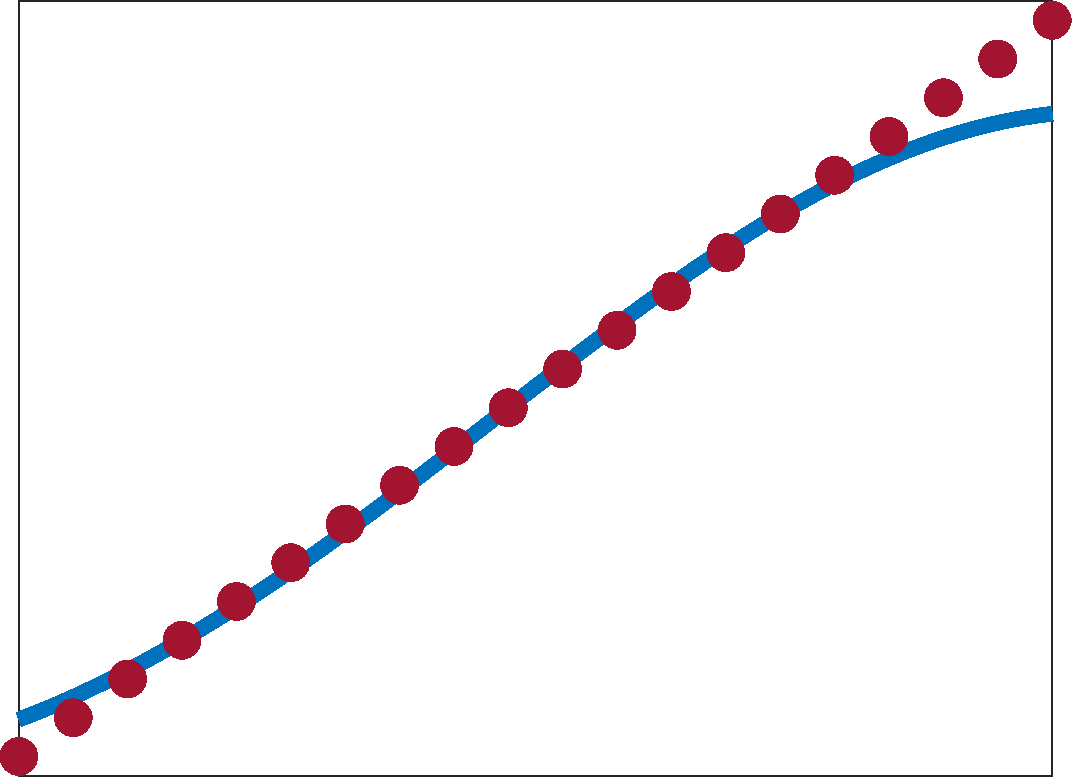
\includegraphics[width=0.16\textwidth]{../src/figures/estimation/gui_rbf}}\qquad
\subfloat[Trigonometric kernel, degree 1.]{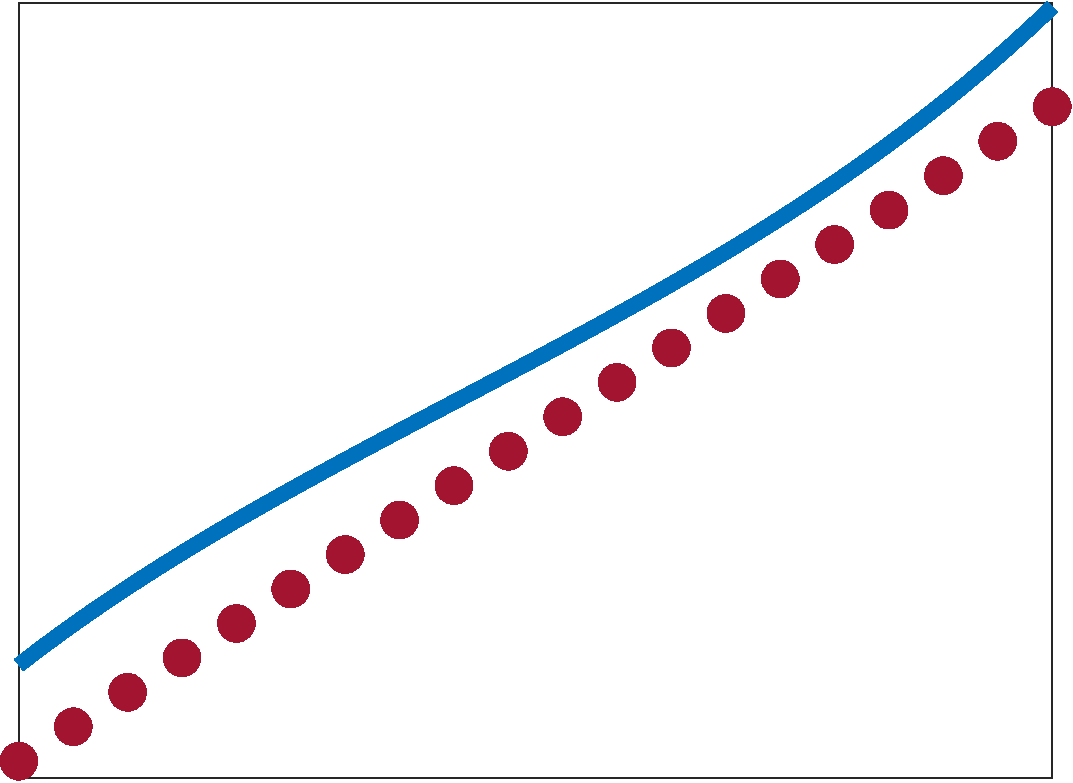
\includegraphics[width=0.16\textwidth]{../src/figures/estimation/gui_trigonometric}}\qquad
\subfloat[Exponential kernel, $\sigma^2=1$.]{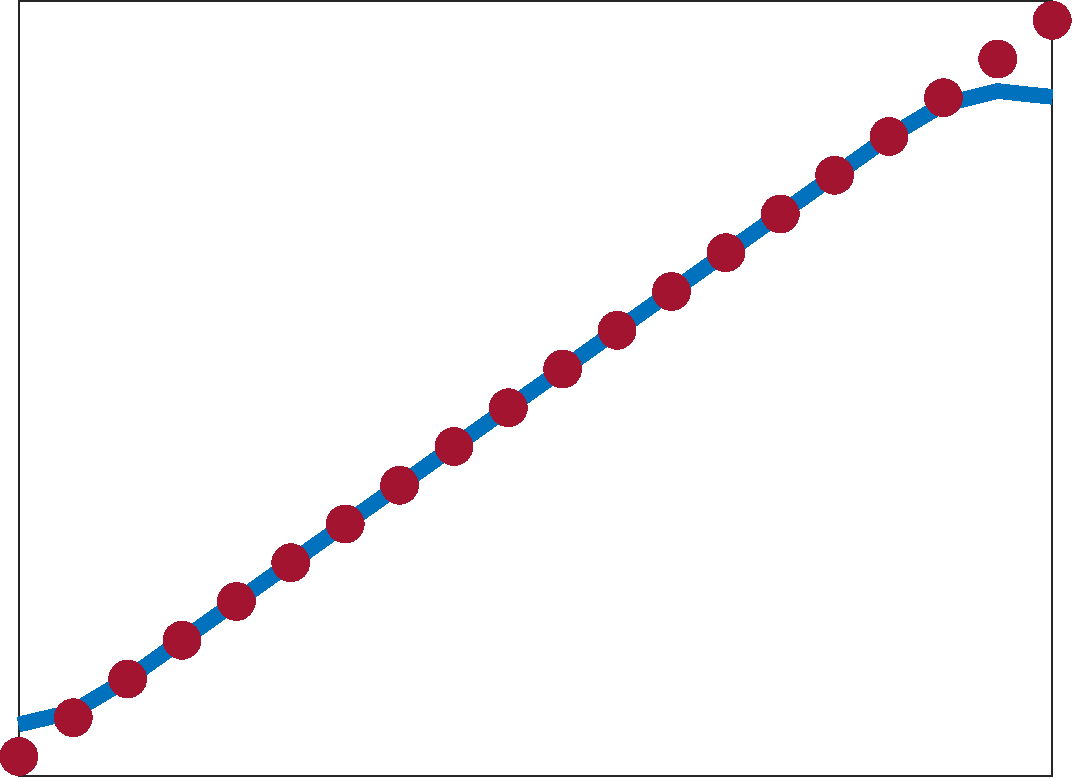
\includegraphics[width=0.16\textwidth]{../src/figures/estimation/gui_exponential}}\qquad
\\
\subfloat[Linear kernel.]{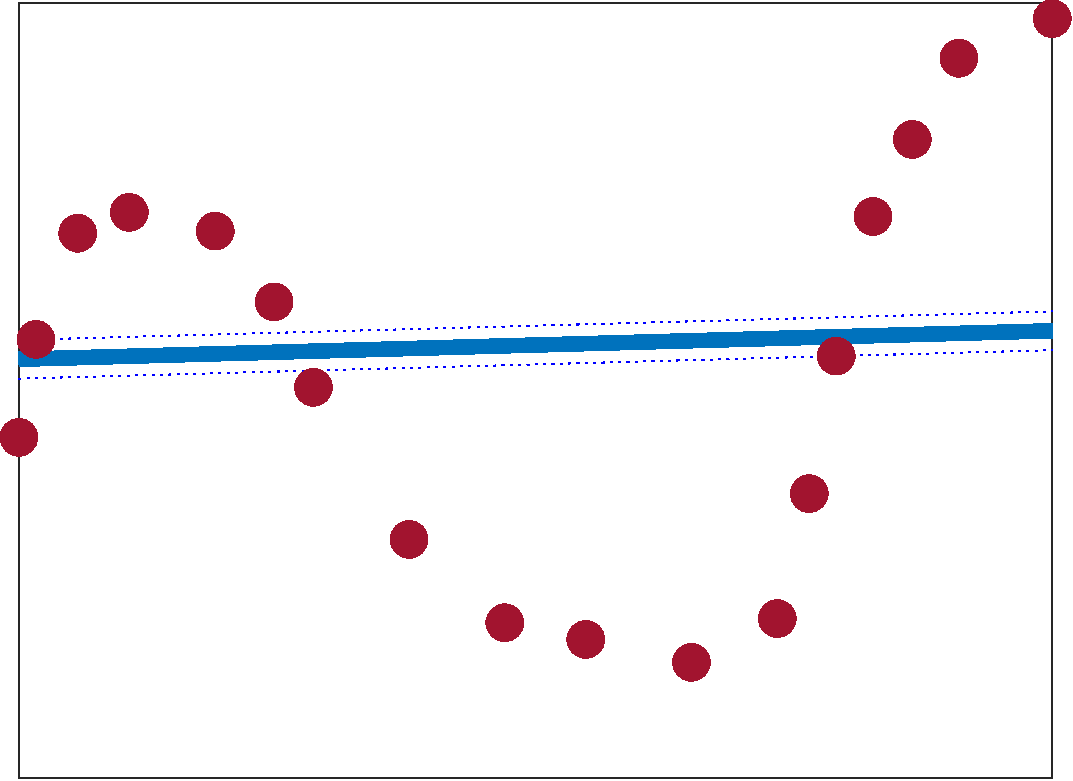
\includegraphics[width=0.16\textwidth]{../src/figures/estimation/gui_nonlinear_linear}}\qquad
\subfloat[Polynomial kernel, $\delta=3$.]{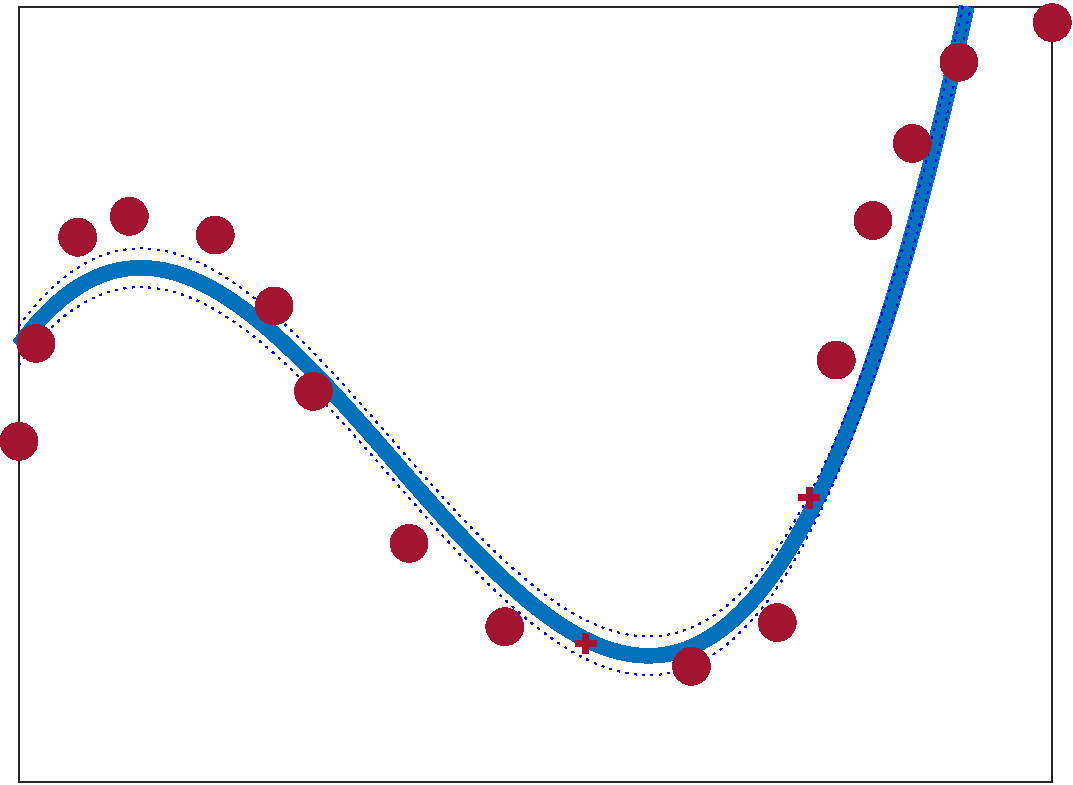
\includegraphics[width=0.16\textwidth]{../src/figures/estimation/gui_nonlinear_polynomial}}\qquad
\subfloat[RBF kernel, $\sigma^2=0.1$.]{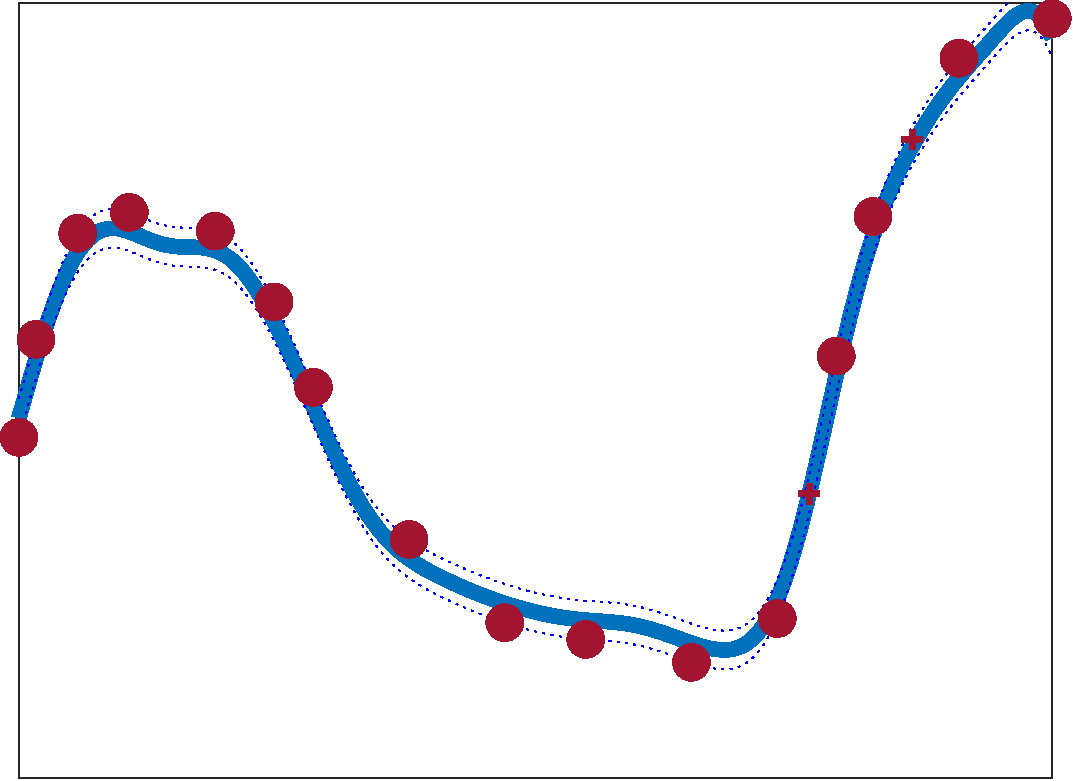
\includegraphics[width=0.16\textwidth]{../src/figures/estimation/gui_nonlinear_rbf}}\qquad
\subfloat[Linear b-spline kernel, degree 5.]{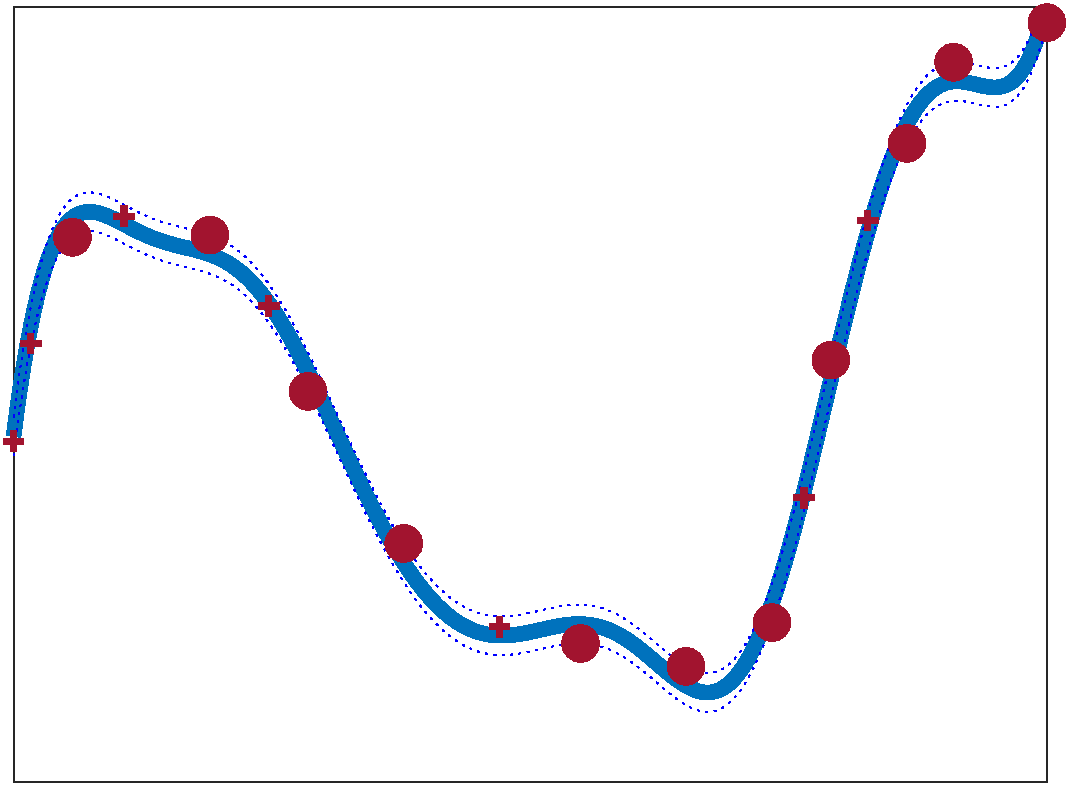
\includegraphics[width=0.16\textwidth]{../src/figures/estimation/gui_nonlinear_bspline}}\qquad
\subfloat[Exponential kernel, $\sigma^2=1.0$.]{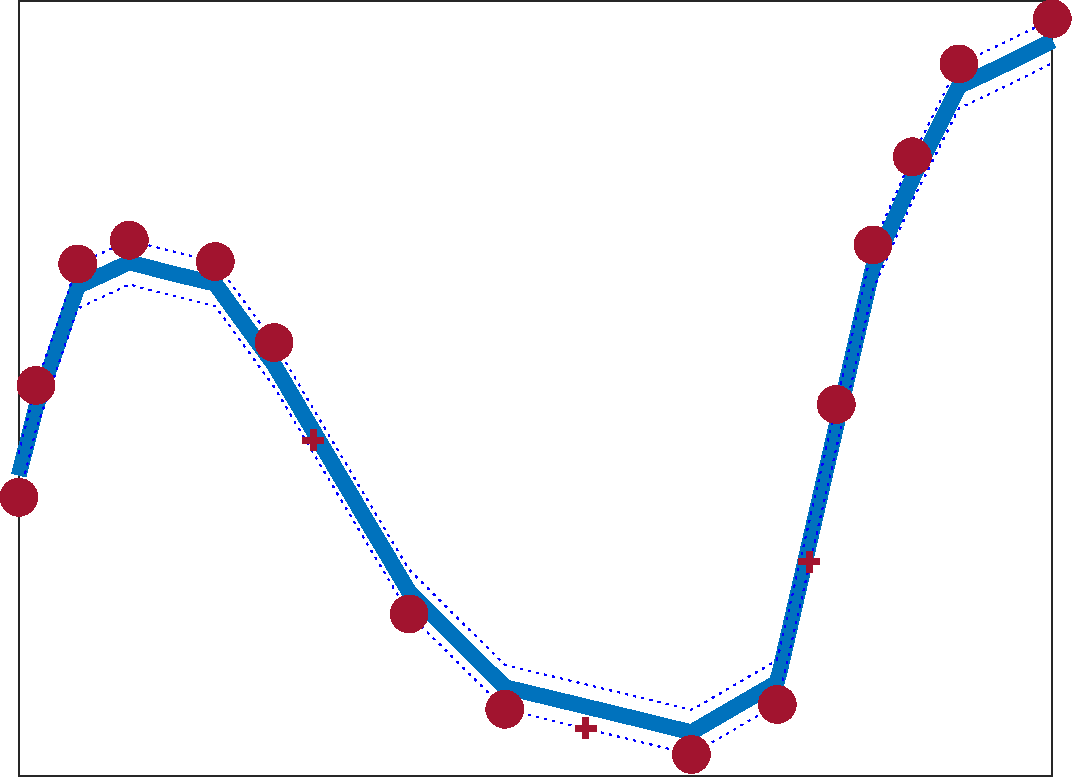
\includegraphics[width=0.16\textwidth]{../src/figures/estimation/gui_nonlinear_exponential}}\qquad
\caption{Visualisation of the results of experiments with various kernels and parameters for two different datasets. In the first row $\epsilon=0$ and \texttt{bound} = 10, in the second one $\epsilon=1$ and \texttt{bound} = 1000. Some of the models are likely to be overfitted though these are just toy examples without any test set.}
\label{functionestimation}
\end{figure}

\fakesubsection{A simple example: the sinc function}{}

Figure \ref{sincestimate} shows the results of LS-SVM regression applied on the \texttt{sinc} function. The mean squared error is lowest for a case that is clearly overfitting. In this case the underlying function is known and it seems reasonable to take $\sigma\in\{0.1,1.0\}$ and, say, $\gamma=10^3$. However, an optimal parameter cannot be found as it depends strongly on the training set.

\par Results of automated tuning are shown hereunder :

\begin{table}[h]
\centering
\begin{tabular}{c|ccc}
\textit{Method} & $\gamma$ & $\sigma^2$ & \textit{mean squared error} \\
\hline
Grid search & 5528319.4668 $\pm$ 54371026.5606 & 0.1239 $\pm$  0.1513 & 0.0104 $\pm$ 0.0001\\
Nelder-Mead & 2329.7378 $\pm$ 2318.2696 & 0.1049 $\pm$ 0.0892 &  0.0104 $\pm$ 0.0001\\
\end{tabular}
\caption{Results of automated tuning strategies (averaged over 40 runs).}
\label{automatedtuning}
\end{table}

The results are comparable to those obtained previously in the context of classification, with a few outliers for $\gamma$. Again, grid search appeared to be slower (185 seconds versus 110 for the simplex method). Some of the models seem to overfit the data a bit.

\begin{figure}[h]
\centering
\subfloat[$\gamma=10,\sigma=0.01,\rho=0.0117$]{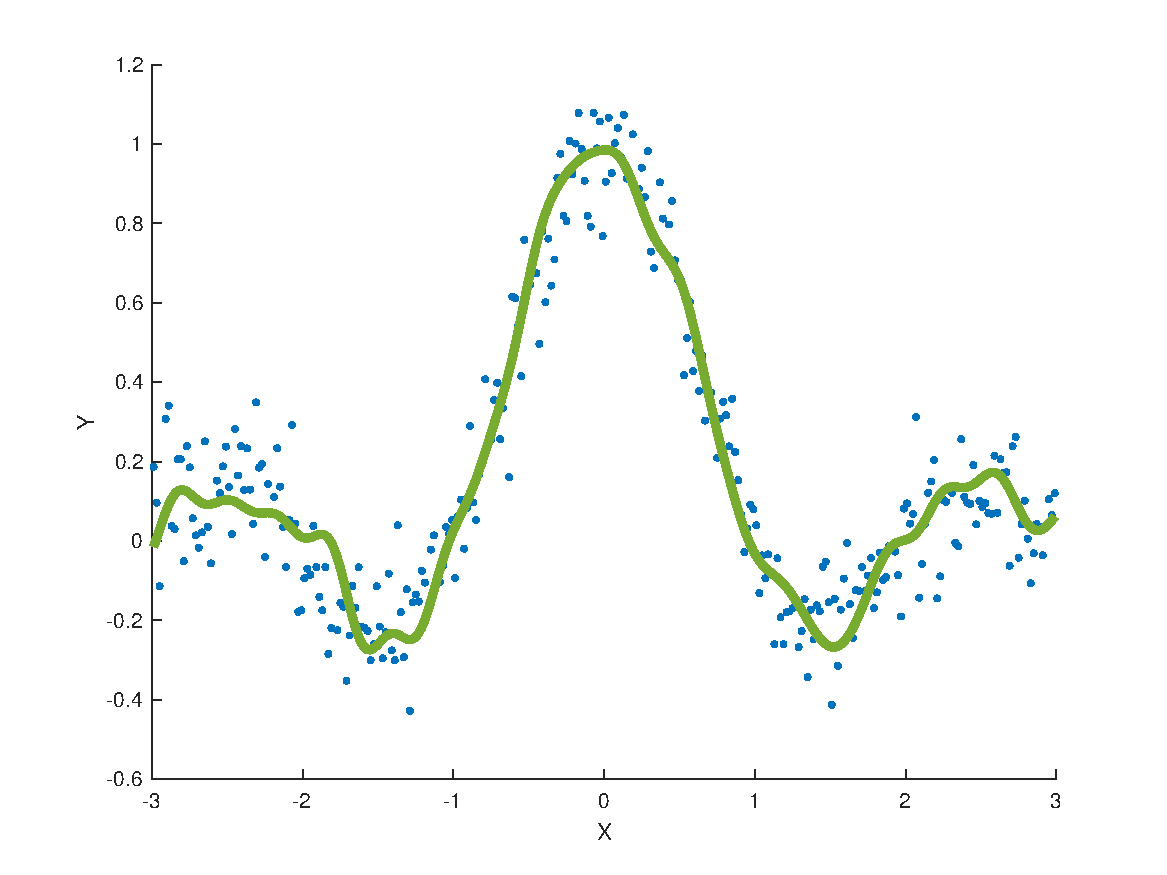
\includegraphics[width=0.3\textwidth]{../src/figures/estimation/regression_1}}\qquad
\subfloat[$\gamma=10,\sigma=1,\rho=0.0296$]{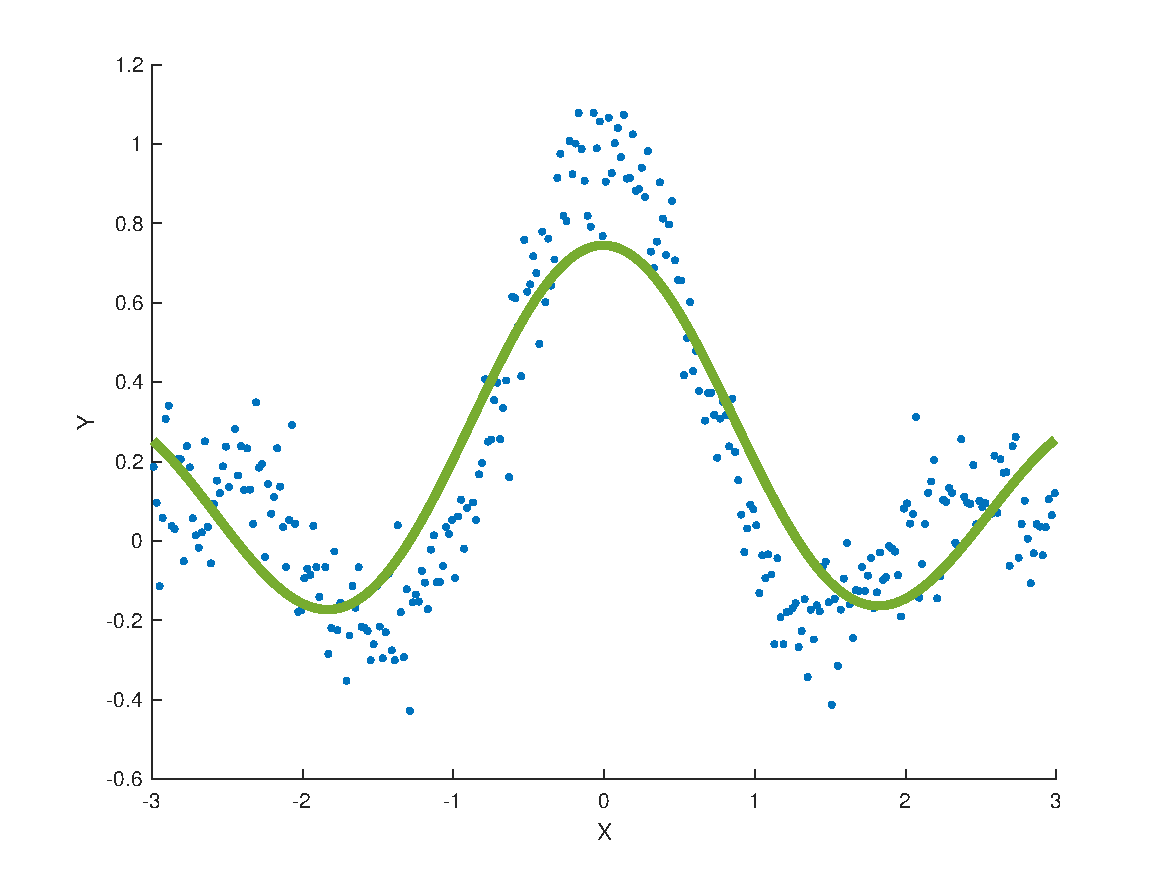
\includegraphics[width=0.3\textwidth]{../src/figures/estimation/regression_2}}\qquad
\subfloat[$\gamma=10,\sigma=100,\rho=0.1273$]{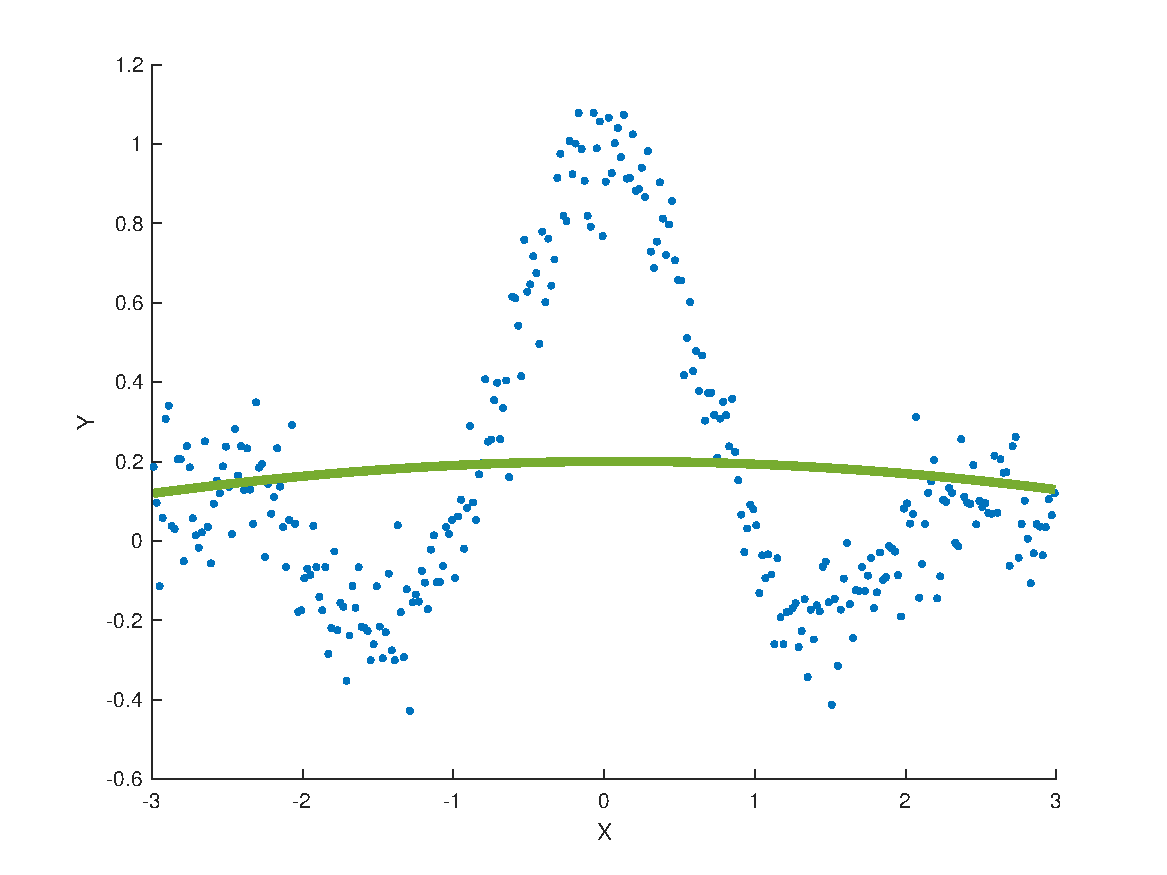
\includegraphics[width=0.3\textwidth]{../src/figures/estimation/regression_3}}\qquad
\\
\subfloat[$\gamma=10^3,\sigma=0.01,\rho=0.0120$]{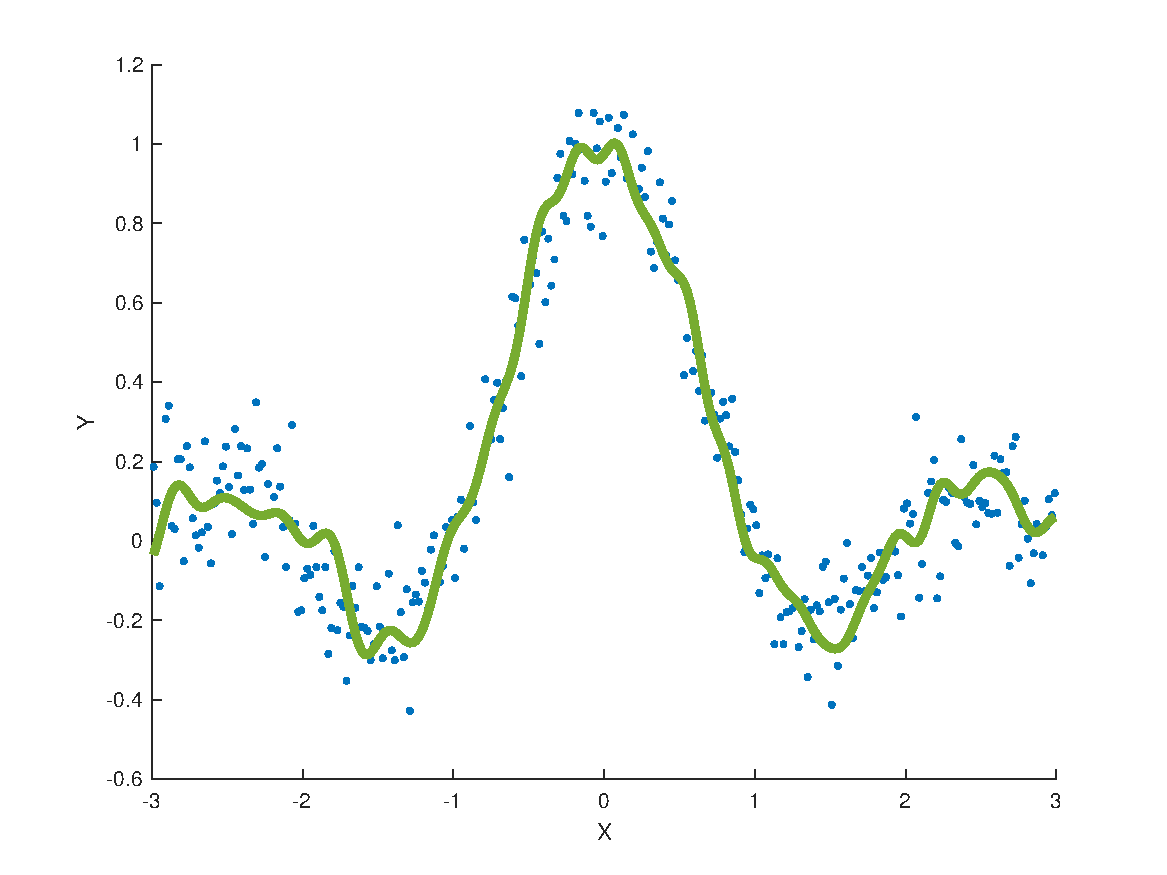
\includegraphics[width=0.3\textwidth]{../src/figures/estimation/regression_4}}\qquad
\subfloat[$\gamma=10^3,\sigma=1,\rho=0.0114$]{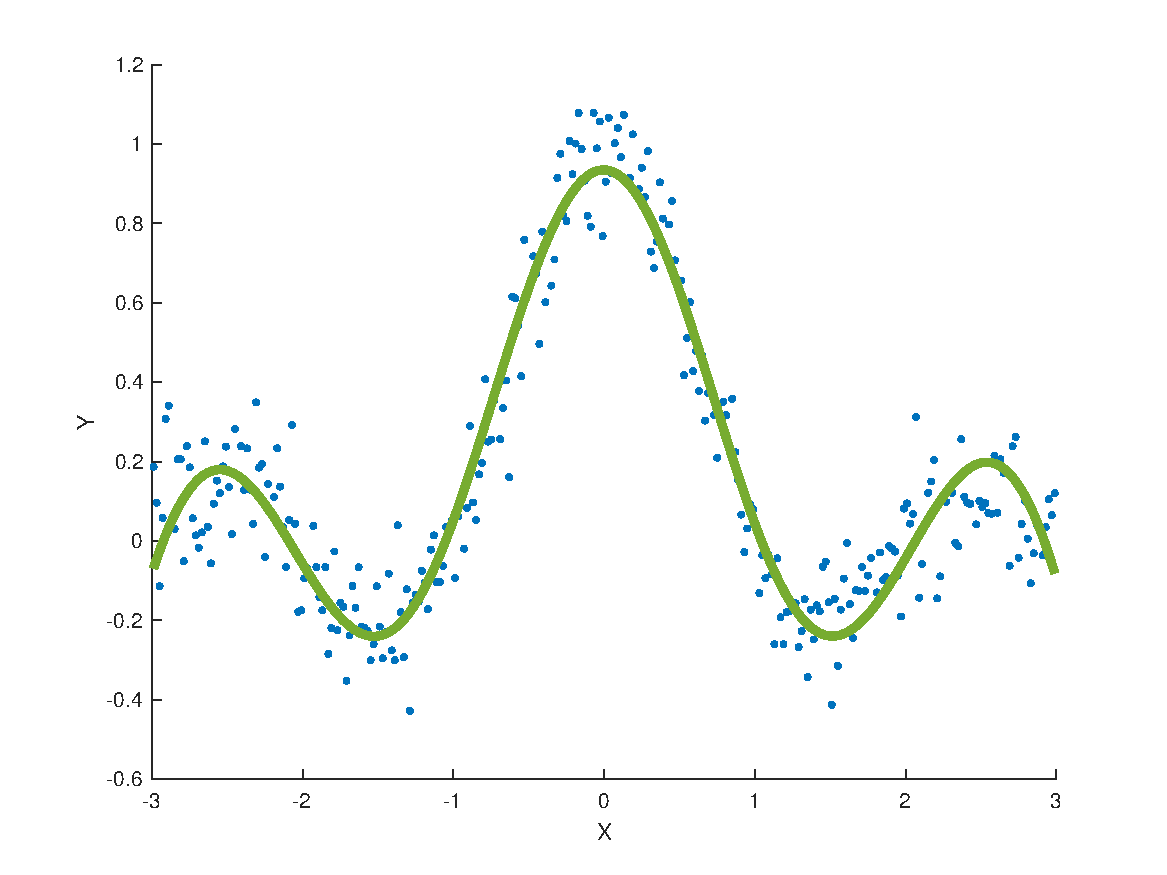
\includegraphics[width=0.3\textwidth]{../src/figures/estimation/regression_5}}\qquad
\subfloat[$\gamma=10^3,\sigma=100,\rho=0.1107$]{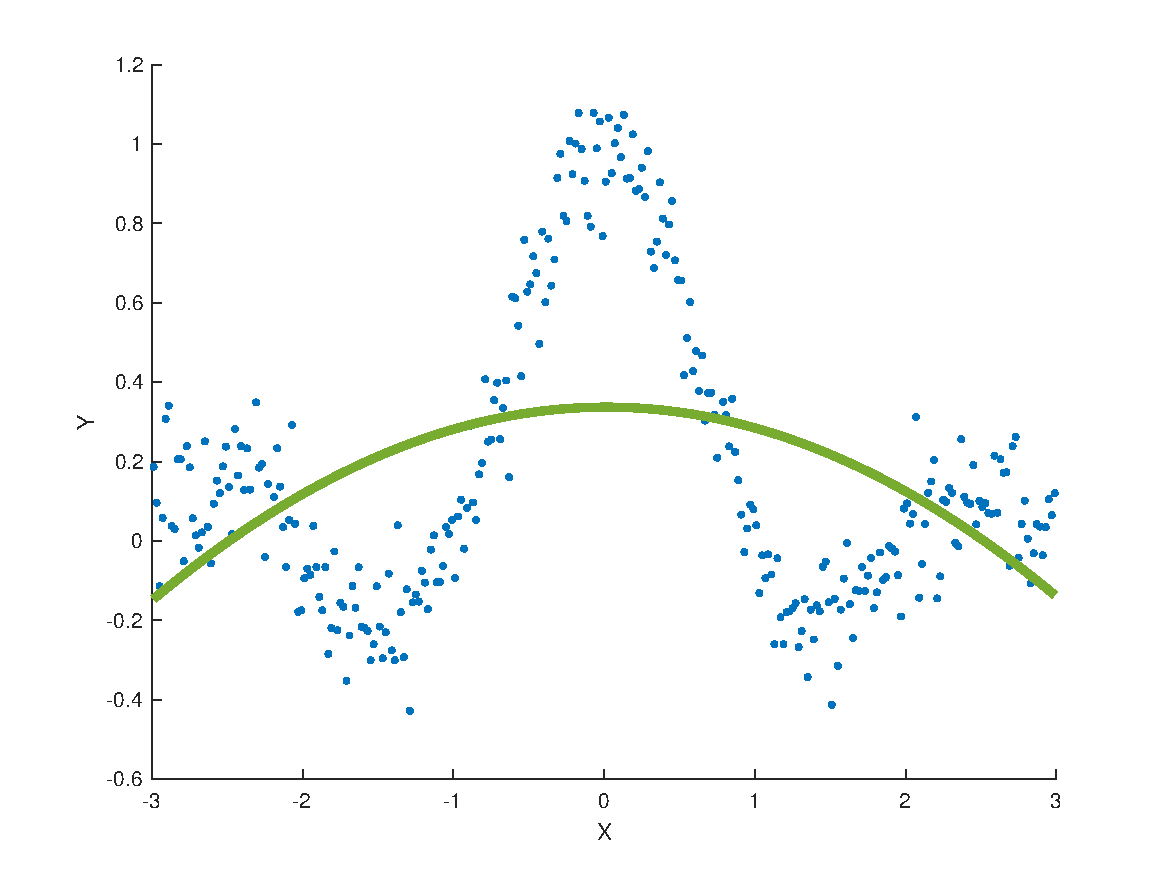
\includegraphics[width=0.3\textwidth]{../src/figures/estimation/regression_6}}\qquad
\\
\subfloat[$\gamma=10^6,\sigma=0.01,\rho=0.0125$]{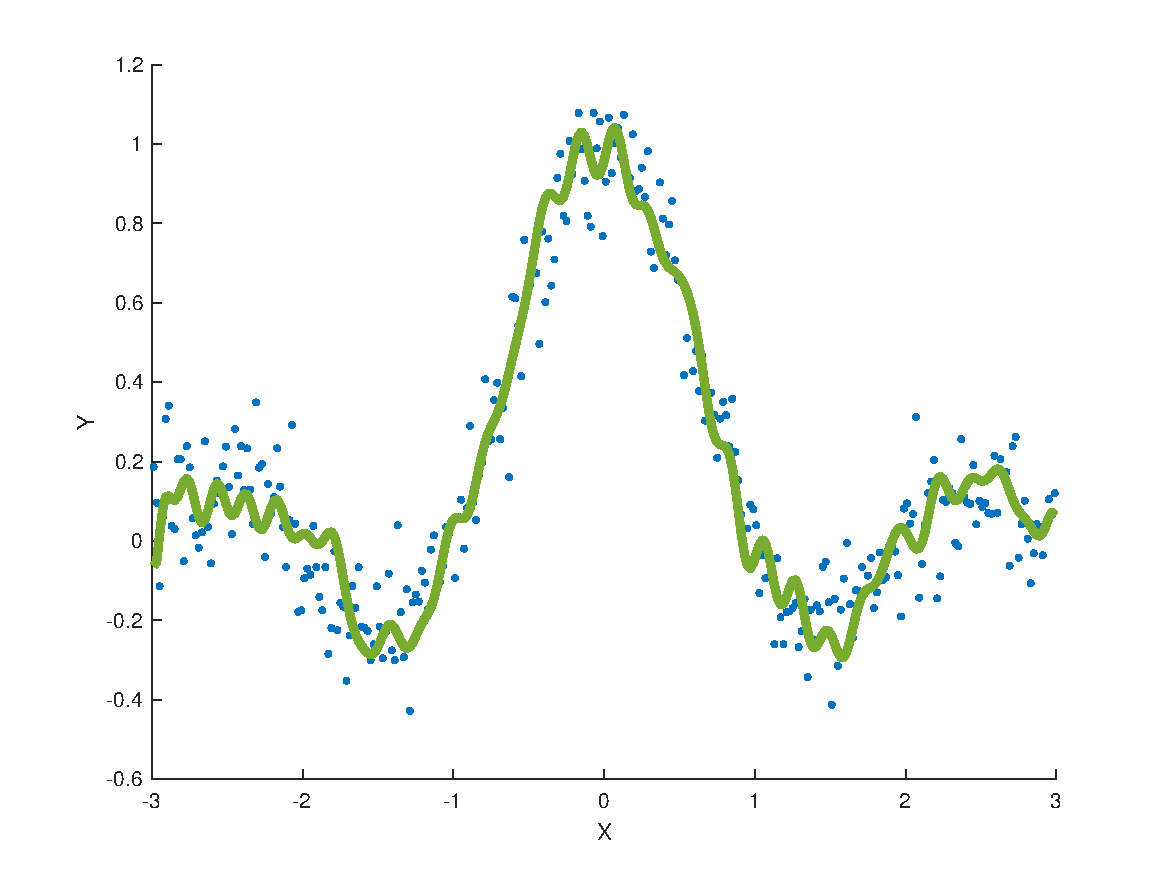
\includegraphics[width=0.3\textwidth]{../src/figures/estimation/regression_7}}\qquad
\subfloat[$\gamma=10^6,\sigma=1,\rho=0.0099$]{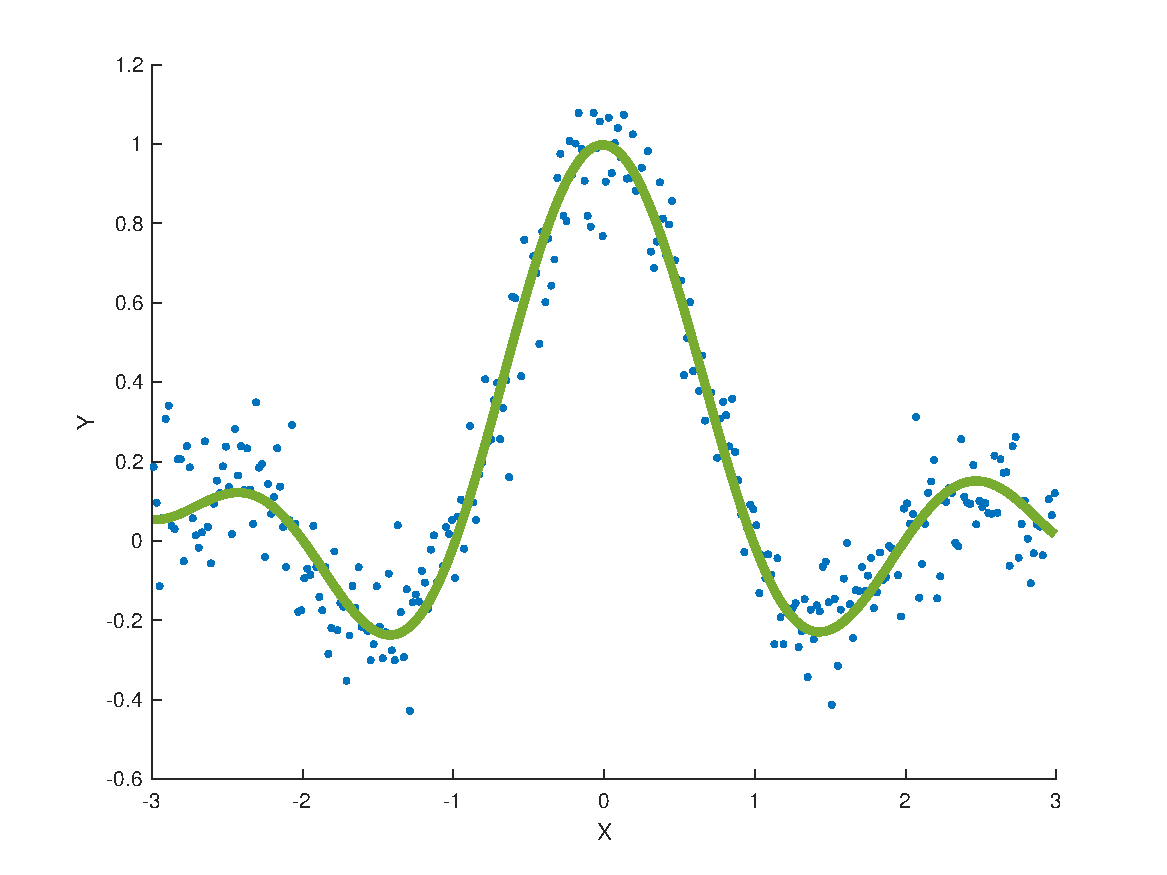
\includegraphics[width=0.3\textwidth]{../src/figures/estimation/regression_8}}\qquad
\subfloat[$\gamma=10^6,\sigma=100,\rho=0.1048$]{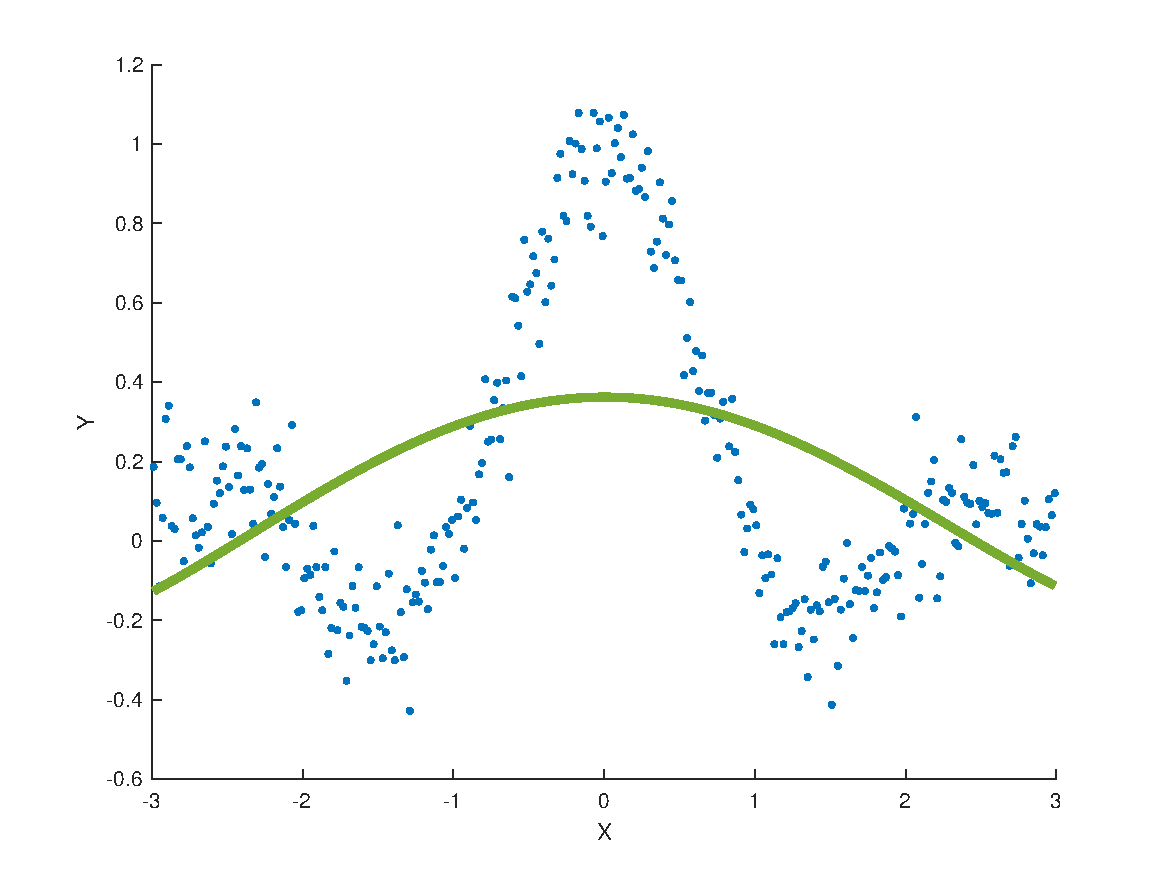
\includegraphics[width=0.3\textwidth]{../src/figures/estimation/regression_9}}\qquad
\caption{Function estimation experiments with the \texttt{sinc} function. Noisy samples are fed to an LS-SVM. The green line is the estimated model, the blue dots represent the test data. $\rho$ is the mean squared error. Small $\sigma$ values make the model fit the noise.}
\label{sincestimate}
\end{figure}

\fakesubsection{Automatic Relevance Determination}{}



\fakesubsection{Robust regression}{}

By applying cross-validation on any subset of the input features one can consider the most promising subset as having the relevant features.

\fakesubsection{Introduction: time series prediction}{}


\fakesubsection{Logmap dataset}{}


\fakesubsection{Santa Fe dataset}{}



